\pdfminorversion=4 % for acroread
%\documentclass[aspectratio=169,t,xcolor={usenames,dvipsnames}]{beamer}
\documentclass[aspectratio=169,t,handout,xcolor={usenames,dvipsnames}]{beamer}
\usepackage{../beamerstyle}
\usepackage{dsfont}
\usepackage{bm}
\usepackage[english]{babel}
\usepackage[utf8]{inputenc}
\usepackage{graphicx}
\usepackage{algorithm}
\usepackage[ruled,vlined,algo2e,linesnumbered]{algorithm2e}
%\usepackage[boxed,vlined]{algorithm2e}
\usepackage{hyperref}
\usepackage{booktabs}
\usepackage{mathtools}

\usepackage{amsmath,amssymb}
\usepackage{listings}
\lstset{frame=lines,framesep=3pt,numbers=left,numberblanklines=false,basicstyle=\ttfamily\small}

\usepackage{subfig}
\usepackage{multicol}
%\usepackage{appendixnumberbeamer}
%
\usepackage{tcolorbox}

\usepackage{pgfplots}
\usepackage{tikz}
\usetikzlibrary{trees} 
\usetikzlibrary{shapes.geometric}
\usetikzlibrary{positioning,shapes,shadows,arrows,calc,mindmap}
\usetikzlibrary{positioning,fadings,through}
\usetikzlibrary{decorations.pathreplacing}
\usetikzlibrary{intersections}
\usetikzlibrary{positioning,fit,calc,shadows,backgrounds}
\pgfdeclarelayer{background}
\pgfdeclarelayer{foreground}
\pgfsetlayers{background,main,foreground}
\tikzstyle{activity}=[rectangle, draw=black, rounded corners, text centered, text width=8em]
\tikzstyle{data}=[rectangle, draw=black, text centered, text width=8em]
\tikzstyle{myarrow}=[->, thick, draw=black]

% Define the layers to draw the diagram
\pgfdeclarelayer{background}
\pgfdeclarelayer{foreground}
\pgfsetlayers{background,main,foreground}

%\usepackage{listings}
%\lstset{numbers=left,
%  showstringspaces=false,
%  frame={tb},
%  captionpos=b,
%  lineskip=0pt,
%  basicstyle=\ttfamily,
%%  extendedchars=true,
%  stepnumber=1,
%  numberstyle=\small,
%  xleftmargin=1em,
%  breaklines
%}

 
\definecolor{blue}{RGB}{0, 74, 153}

\usetheme{Boadilla}
%\useinnertheme{rectangles}
\usecolortheme{whale}
\setbeamercolor{alerted text}{fg=blue}
\useoutertheme{infolines}
\setbeamertemplate{navigation symbols}{\vspace{-5pt}} % to lower the logo
\setbeamercolor{date in head/foot}{bg=white} % blue
\setbeamercolor{date in head/foot}{fg=white}
\setbeamercolor{author  in head/foot}{bg=white} %blue
\setbeamercolor{title in head/foot}{bg=white} % blue
\setbeamercolor{title}{fg=white, bg=blue}
\setbeamercolor{block title}{fg=white,bg=blue}
\setbeamercolor{block body}{bg=blue!10}
\setbeamercolor{frametitle}{fg=white, bg=blue}
\setbeamercovered{invisible}

\makeatletter
\setbeamertemplate{footline}
{
  \leavevmode%
  \hbox{%
  \begin{beamercolorbox}[wd=.333333\paperwidth,ht=2.25ex,dp=1ex,center]{author in head/foot}%
%    \usebeamerfont{author in head/foot}\insertshortauthor
  \end{beamercolorbox}%
  \begin{beamercolorbox}[wd=.333333\paperwidth,ht=2.25ex,dp=1ex,center]{title in head/foot}%
    \usebeamerfont{title in head/foot}\insertshorttitle
  \end{beamercolorbox}%
  \begin{beamercolorbox}[wd=.333333\paperwidth,ht=2.25ex,dp=1ex,right]{date in head/foot}%
    \usebeamerfont{date in head/foot}\insertshortdate{}\hspace*{2em}
%    \insertframenumber\hspace*{2ex} 
  \end{beamercolorbox}}%
  \vskip0pt%
}
\makeatother

%\pgfdeclareimage[height=1.2cm]{automl}{images/logos/automl.png}
%\pgfdeclareimage[height=1.2cm]{freiburg}{images/logos/freiburg}

%\logo{\pgfuseimage{freiburg}}

\renewcommand{\comment}[1]{
	\noindent
	%\vspace{0.25cm}
	{\color{red}{\textbf{TODO:} #1}}
	%\vspace{0.25cm}
}
\newcommand{\notefh}[1]{\textcolor{red}{\textbf{FH:} #1}}
\renewcommand{\comment}[1]{}
\newcommand{\hide}[1]{}
\newcommand{\cemph}[2]{\emph{\textcolor{#1}{#2}}}

\newcommand{\lit}[1]{{\footnotesize\color{black!60}[#1]}}

\newcommand{\litw}[1]{{\footnotesize\color{blue!20}[#1]}}


\newcommand{\myframe}[2]{\begin{frame}[c]{#1}#2\end{frame}}
\newcommand{\myframetop}[2]{\begin{frame}{#1}#2\end{frame}}
\newcommand{\myit}[1]{\begin{itemize}#1\end{itemize}}
\newcommand{\myblock}[2]{\begin{block}{#1}#2\end{block}}


\newcommand{\votepurple}[1]{\textcolor{Purple}{$\bigstar$}}
\newcommand{\voteyellow}[1]{\textcolor{Goldenrod}{$\bigstar$}}
\newcommand{\voteblue}[1]{\textcolor{RoyalBlue}{$\bigstar$}}
\newcommand{\votepink}[1]{\textcolor{Pink}{$\bigstar$}}

\newcommand{\diff}{\mathop{}\!\mathrm{d}}
\newcommand{\refstyle}[1]{{\small{\textcolor{gray}{#1}}}}
\newcommand{\hands}[0]{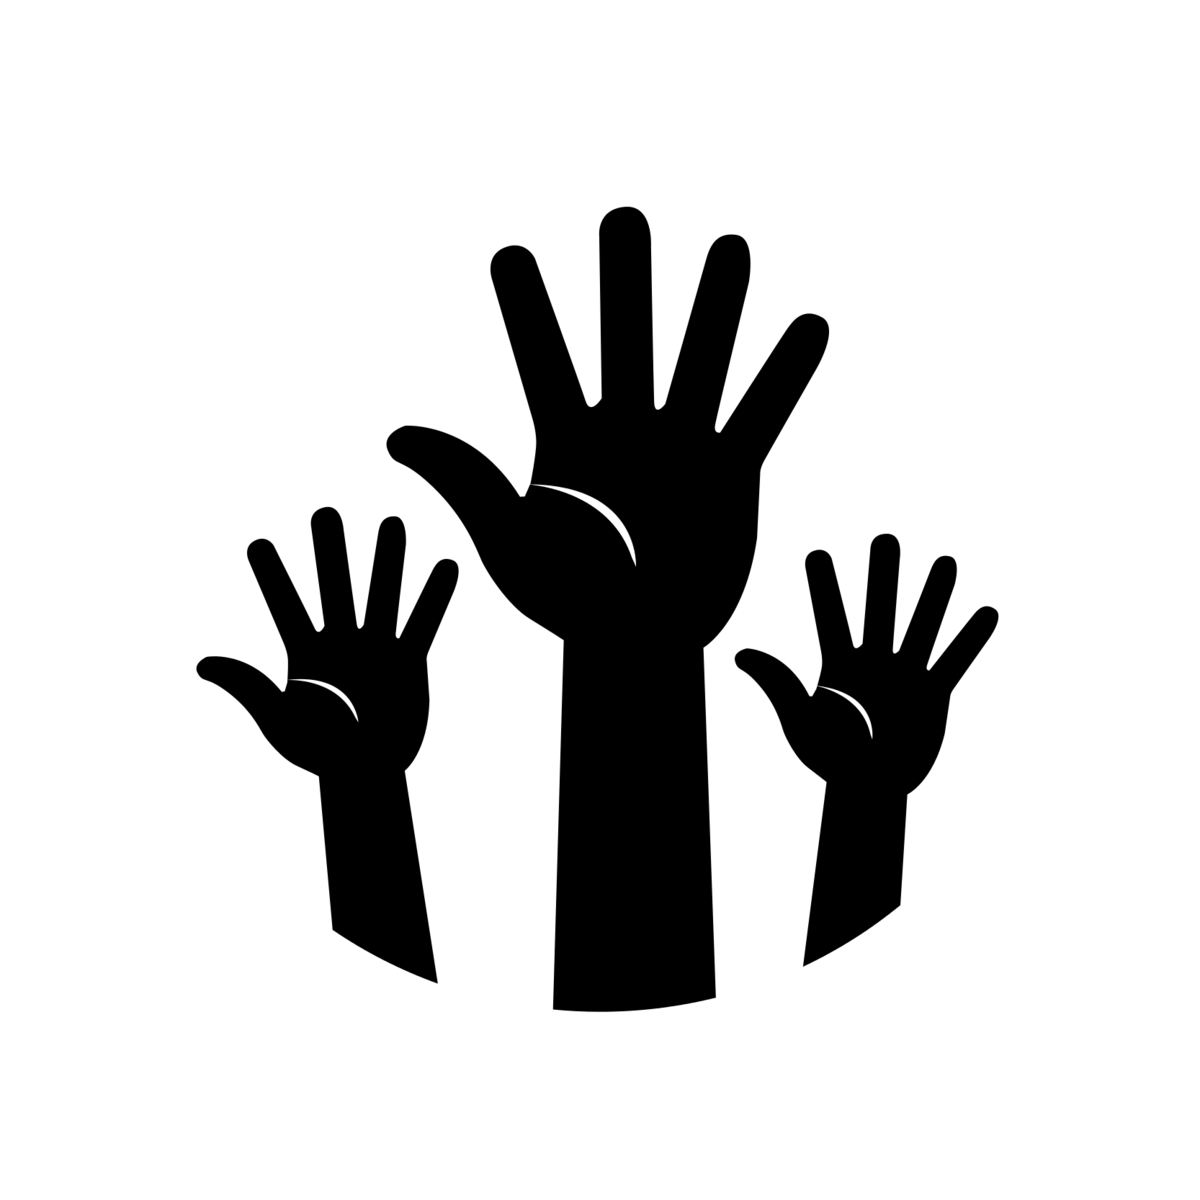
\includegraphics[height=1.5em]{images/hands}}
\newcommand{\transpose}[0]{{\textrm{\tiny{\sf{T}}}}}
\newcommand{\norm}{{\mathcal{N}}}
\newcommand{\cutoff}[0]{\kappa}
\newcommand{\instD}[0]{\dataset}
\newcommand{\insts}[0]{\mathcal{I}}
\newcommand{\inst}[0]{i}
\newcommand{\instI}[1]{i^{(#1)}}

% Iteration specific instance of variable/function/anything
% Introduced in the BO section, but moved up here to make it available within other macros
\newcommand{\iter}[2][\bocount]{{#2}^{(#1)}}

%--------HPO parameter macros-----------

% Parameter Configuration Space
\newcommand{\pcs}[0]{\pmb{\Lambda}}

% ???
\newcommand{\bx}[0]{\conf}

% Parameter Configuration
\newcommand{\conf}[0]{\pmb{\lambda}}

% Final Configuration
\newcommand{\finconf}[0]{\pmb{\hat{\lambda}}}

% Configuration corresponding to a given iteration -- better use \iter!
\newcommand{\confI}[1]{{\conf}^{(#1)}}

% Default Configuration
\newcommand{\defconf}[0]{{\conf}_{\text{def}}}

% Incumbent Configuration
\newcommand{\incumbent}[1][\bocount]{\iter[#1]{\finconf}}

% Optimal Configuration
\newcommand{\optconf}[0]{{\conf}^*}

% Configuration Space
\newcommand{\confs}[0]{\pcs}

%----------------------------------------

%\newcommand{\vlambda}[0]{\bm{\lambda}}
%\newcommand{\vLambda}[0]{\bm{\Lambda}}
\newcommand{\dataset}[0]{\mathcal{D}}
\newcommand{\datasets}[0]{\mathbf{D}}
\newcommand{\loss}[0]{L}
\newcommand{\risk}{\mathcal{R}}
\newcommand{\riske}{\mathcal{R}_{\text{emp}}}
\newcommand{\cost}[0]{c}
\newcommand{\costI}[1]{c^{(#1)}}

% Gaussian Process
\newcommand{\gp}{\mathcal{G}}
% Family of Objective Functions
\newcommand{\objF}{F}

%---------------BO Macros------------------

% BO loop counter
\newcommand{\bocount}{t}
% BO loop counter max, the counter runs from 1 to this value
\newcommand{\bobudget}{T}
% BO loop observation
\newcommand{\obs}[1][\conf]{\cost({#1})}
% BO loop observation space
\newcommand{\obsspace}{\mathcal{Y}}
% BO loop next observation
\newcommand{\bonextobs}{\obs[\iter{\conf}]}
% Acquisition Function, no args
\newcommand{\acq}{u}
% Standard Normal PDF
\newcommand{\pdf}{\phi}
% Standard Normal CDF
\newcommand{\cdf}{\Phi}
% Mean
\newcommand{\mean}{\mu}
% Standard Deviation
\newcommand{\stddev}{\sigma}
% Variance
\newcommand{\variance}{\sigma^2}
% Noise
\newcommand{\noise}{\nu}
% BO loop next selected sample
\newcommand{\bonextsample}{\confI{\bocount}}

% Single hyperparameter
\newcommand{\hyperparam}{\lambda}

% Single hyperparameter within a hyperparameter configuration
\newcommand{\hyperparami}[1][i]{{\hyperparam}_#1}

% Full definition of final configuration
\newcommand{\finconffull}{\incumbent[\bobudget]}

% Dataset
\newcommand{\datasetHPO}{{\dataset}_{HPO}}

% Dataset definition
\newcommand{\datasetHPOdef}{{\langle \bonextsample,\,\bonextobs \rangle}_{\bocount=1}^{\bobudget}}

% Double Display Fraction, forces large displays for everything in numerator and denominator
\newcommand\ddfrac[2]{\frac{\displaystyle #1}{\displaystyle #2}}

% Conditional Probability "Given That" Relation, source:https://tex.stackexchange.com/a/141685/205886
\newcommand\given[1][]{\:#1\vert\:}

% Expectation as a math operator
\DeclareMathOperator*{\E}{\mathbb{E}}

% Citation 
\newcommand{\source}[1]{
    \begin{flushright}
    	Source: \lit{#1}
    \end{flushright}
}
%-------------------------------------------

%Real numbers set
\newcommand{\realnum}{\mathbb{R}}
%Configuration space - do not use
%\newcommand{\configspace}{\Theta}
%Instances - do not use
%\newcommand{\instances}{\mathcal{I}}
%Expected value
\newcommand{\expectation}{\mathbb{E}}
%Kernel
\newcommand{\kernel}{\kappa}
%Constraint function
\newcommand{\constraintf}{c}
%Normal distribution
\newcommand{\normaldist}{\mathcal{N}}

% \renewcommand{\vec}[1]{\mathbf{#1}}
\newcommand{\hist}[0]{\dataset_{\text{Hist}}}
\newcommand{\param}[0]{p}
\newcommand{\algo}[0]{\mathcal{A}}
\newcommand{\algos}[0]{\mathbf{A}}
%\newcommand{\nn}[0]{N}
\newcommand{\feats}[0]{\mathcal{X}_{\text{meta}}}
\newcommand{\feat}[0]{\x_{\text{meta}}}
%\newcommand{\cluster}[0]{\vec{h}}
%\newcommand{\clusters}[0]{\vec{H}}
\newcommand{\perf}[0]{\mathbb{R}}
%\newcommand{\surro}[0]{\mathcal{S}}
\newcommand{\surro}[0]{\hat{\cost}}
\newcommand{\func}[0]{f}
\newcommand{\epm}[0]{\surro}
\newcommand{\portfolio}[0]{\mathbf{P}}
\newcommand{\schedule}[0]{\mathcal{S}}

% Machine Learning
\newcommand{\mdata}[0]{\dataset_{\text{meta}}}
\newcommand{\datasettrain}[0]{\dataset_{\text{train}}}
\newcommand{\datasetval}[0]{\dataset_{\text{val}}}
\newcommand{\datasettest}[0]{\dataset_{\text{test}}}
\newcommand{\x}[0]{\mathbf{x}}
\newcommand{\y}[0]{y}
\newcommand{\xI}[1]{\mathbf{x}^{(#1)}}
\newcommand{\yI}[1]{y^{(#1)}}
\newcommand{\fx}{f(\mathbf{x})}  % f(x), continuous prediction function
\newcommand{\Hspace}{\mathcal{H}} % hypothesis space where f is from
\newcommand{\fh}{\hat{f}}       % f hat, estimated prediction function

% Deep Learning
\newcommand{\weights}[0]{\theta}
\newcommand{\metaweights}[0]{\phi}


% reinforcement learning
\newcommand{\policies}[0]{\mathbf{\Pi}}
\newcommand{\policy}[0]{\pi}
\newcommand{\actionRL}[0]{a}
\newcommand{\stateRL}[0]{s}
\newcommand{\statesRL}[0]{\mathcal{S}}
\newcommand{\rewardRL}[0]{r}
\newcommand{\rewardfuncRL}[0]{\mathcal{R}}

\RestyleAlgo{algoruled}
\DontPrintSemicolon
\LinesNumbered
\SetAlgoVlined
\SetFuncSty{textsc}

\SetKwInOut{Input}{Input}
\SetKwInOut{Output}{Output}
\SetKw{Return}{return}

%\newcommand{\changed}[1]{{\color{red}#1}}

%\newcommand{\citeN}[1]{\citeauthor{#1}~(\citeyear{#1})}

\renewcommand{\vec}[1]{\mathbf{#1}}
\DeclareMathOperator*{\argmin}{arg\,min}
\DeclareMathOperator*{\argmax}{arg\,max}

%\newcommand{\aqme}{\textit{AQME}}
%\newcommand{\aslib}{\textit{ASlib}}
%\newcommand{\llama}{\textit{LLAMA}}
%\newcommand{\satzilla}{\textit{SATzilla}}
%\newcommand{\satzillaY}[1]{\textit{SATzilla'{#1}}}
%\newcommand{\snnap}{\textit{SNNAP}}
%\newcommand{\claspfolioTwo}{\textit{claspfolio~2}}
%\newcommand{\flexfolio}{\textit{FlexFolio}}
%\newcommand{\claspfolioOne}{\textit{claspfolio~1}}
%\newcommand{\isac}{\textit{ISAC}}
%\newcommand{\eisac}{\textit{EISAC}}
%\newcommand{\sss}{\textit{3S}}
%\newcommand{\sunny}{\textit{Sunny}}
%\newcommand{\ssspar}{\textit{3Spar}}
%\newcommand{\cshc}{\textit{CSHC}}
%\newcommand{\cshcpar}{\textit{CSHCpar}}
%\newcommand{\measp}{\textit{ME-ASP}}
%\newcommand{\aspeed}{\textit{aspeed}}
%\newcommand{\autofolio}{\textit{AutoFolio}}
%\newcommand{\cedalion}{\textit{Cedalion}}
\newcommand{\fanova}{\textit{fANOVA}}
\newcommand{\sbs}{\textit{SB}}
\newcommand{\oracle}{\textit{VBS}}

% like approaches
\newcommand{\claspfoliolike}[1]{\texttt{claspfolio-#1-like}}
\newcommand{\satzillalike}[1]{\texttt{SATzilla'#1-like}}
\newcommand{\isaclike}{\texttt{ISAC-like}}
\newcommand{\ssslike}{\texttt{3S-like}}
\newcommand{\measplike}{\texttt{ME-ASP-like}}

\newcommand{\irace}{\textit{I/F-race}}
\newcommand{\gga}{\textit{GGA}}
\newcommand{\smac}{\textit{SMAC}}
\newcommand{\paramils}{\textit{ParamILS}}
\newcommand{\spearmint}{\textit{Spearmint}}
\newcommand{\tpe}{\textit{TPE}}


\usepackage{pifont}
\newcommand{\itarrow}{\mbox{\Pisymbol{pzd}{229}}}
\newcommand{\ithook}{\mbox{\Pisymbol{pzd}{52}}}
\newcommand{\itcross}{\mbox{\Pisymbol{pzd}{56}}}
\newcommand{\ithand}{\mbox{\raisebox{-1pt}{\Pisymbol{pzd}{43}}}}

%\DeclareMathOperator*{\argmax}{arg\,max}

\newcommand{\ie}{{\it{}i.e.\/}}
\newcommand{\eg}{{\it{}e.g.\/}}
\newcommand{\cf}{{\it{}cf.\/}}
\newcommand{\wrt}{\mbox{w.r.t.}}
\newcommand{\vs}{{\it{}vs\/}}
\newcommand{\vsp}{{\it{}vs\/}}
\newcommand{\etc}{{\copyedit{etc.}}}
\newcommand{\etal}{{\it{}et al.\/}}

\newcommand{\pscProc}{{\bf procedure}}
\newcommand{\pscBegin}{{\bf begin}}
\newcommand{\pscEnd}{{\bf end}}
\newcommand{\pscEndIf}{{\bf endif}}
\newcommand{\pscFor}{{\bf for}}
\newcommand{\pscEach}{{\bf each}}
\newcommand{\pscThen}{{\bf then}}
\newcommand{\pscElse}{{\bf else}}
\newcommand{\pscWhile}{{\bf while}}
\newcommand{\pscIf}{{\bf if}}
\newcommand{\pscRepeat}{{\bf repeat}}
\newcommand{\pscUntil}{{\bf until}}
\newcommand{\pscWithProb}{{\bf with probability}}
\newcommand{\pscOtherwise}{{\bf otherwise}}
\newcommand{\pscDo}{{\bf do}}
\newcommand{\pscTo}{{\bf to}}
\newcommand{\pscOr}{{\bf or}}
\newcommand{\pscAnd}{{\bf and}}
\newcommand{\pscNot}{{\bf not}}
\newcommand{\pscFalse}{{\bf false}}
\newcommand{\pscEachElOf}{{\bf each element of}}
\newcommand{\pscReturn}{{\bf return}}

%\newcommand{\param}[1]{{\sl{}#1}}
\newcommand{\var}[1]{{\it{}#1}}
\newcommand{\cond}[1]{{\sf{}#1}}
%\newcommand{\state}[1]{{\sf{}#1}}
%\newcommand{\func}[1]{{\sl{}#1}}
\newcommand{\set}[1]{{\Bbb #1}}
%\newcommand{\inst}[1]{{\tt{}#1}}
\newcommand{\myurl}[1]{{\small\sf #1}}

\newcommand{\Nats}{{\Bbb N}}
\newcommand{\Reals}{{\Bbb R}}
\newcommand{\extset}[2]{\{#1 \; | \; #2\}}

\newcommand{\vbar}{$\,\;|$\hspace*{-1em}\raisebox{-0.3mm}{$\,\;\;|$}}
\newcommand{\vendbar}{\raisebox{+0.4mm}{$\,\;|$}}
\newcommand{\vend}{$\,\:\lfloor$}


\newcommand{\goleft}[2][.7]{\parbox[t]{#1\linewidth}{\strut\raggedright #2\strut}}
\newcommand{\rightimage}[2][.3]{\mbox{}\hfill\raisebox{1em-\height}[0pt][0pt]{\includegraphics[width=#1\linewidth]{#2}}\vspace*{-\baselineskip}}





\newcommand{\inducer}{\mathcal{I}}
\newcommand{\R}{\mathds{R}}

%The following might look confusing but allows us to switch the notation of the optimization problem independently from the notation of the hyper parameter optimization
\newcommand{\xx}{\conf} %x of the optimizer
\newcommand{\xxi}[1][i]{\conf_{#1}} %i-th component of xx (not confuse with i-th individual)
\newcommand{\XX}{\pcs} %search space / domain of f
\newcommand{\f}{\cost} %objective function

\newenvironment{blocki}[1] % itemize block
{
 \begin{block}{#1}\begin{itemize}
}
{
\end{itemize}\end{block}
}

\title[AutoML: Hyperparameter Optimization]{AutoML: Hyperparameter Optimization}
%\subtitle{Overview for this Week} %To be defined in source!
%TODO: change authors!
\author[Marius Lindauer]{\underline{Bernd Bischl} \and Frank Hutter \and Lars Kotthoff\newline \and Marius Lindauer \and Joaquin Vanschoren}
\institute{}
\date{}


\usepackage[normalem]{ulem}
\usepackage{pifont}
\usepackage{relsize}
\renewcommand{\lit}[1]{{\smaller\color{black!60}[#1]}}
\subtitle{Wrap Up}


\begin{document}

\maketitle


%----------------------------------------------------------------------
%----------------------------------------------------------------------

\begin{frame}{From HPO to AutoML}
  So far we covered
  \begin{itemize}
    \item Mechanisms to select ML algorithms for a data set (algorithm selection)
    \item HPO as black-box optimization
    \begin{itemize}
      \item Grid- and random search, EAs, BO
    \end{itemize}
    \item HPO as a grey box problem
    \begin{itemize}
      \item Hyperband, BOHB
    \end{itemize}
    \item Neural Architecture Search (NAS)
    \begin{itemize}
      \item One-Shot approaches, DART
    \end{itemize}
    \item Dynamic algorithm configuration (learning to learn)
    \begin{itemize}
      \item Adapt configuration during training
    \end{itemize}
  \end{itemize}  
\end{frame}

\begin{frame}{From HPO to AutoML}
    \begin{center}
      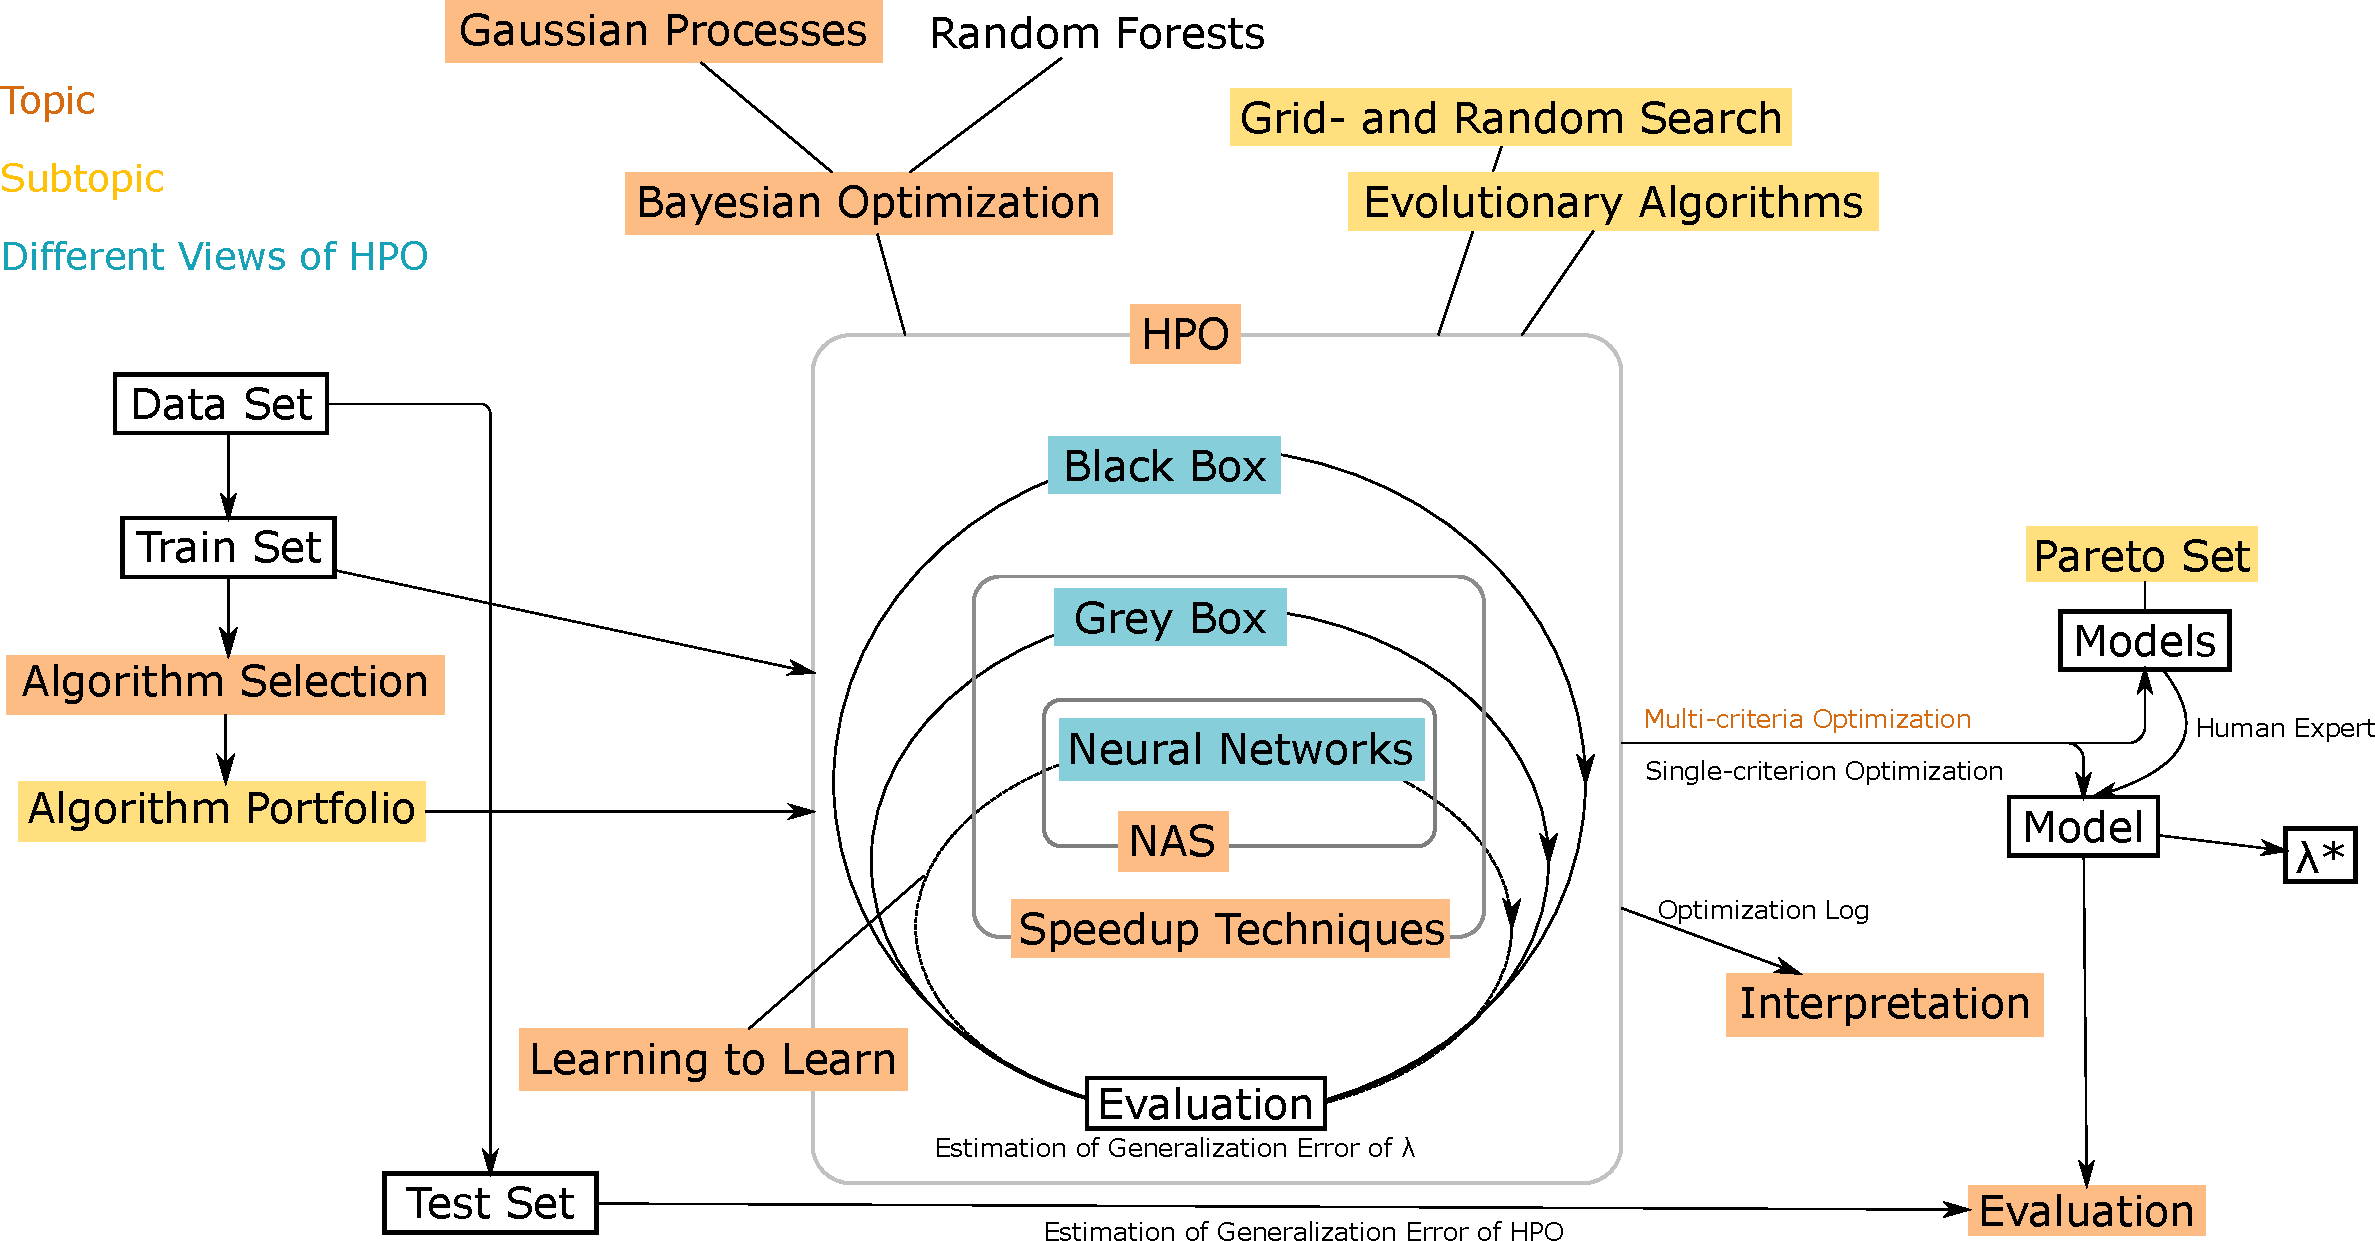
\includegraphics[width = 0.9\linewidth]{images/drawing.pdf}  
    \end{center}
\end{frame}

\section{The Missing Building Blocks}

\begin{frame}{What is missing?}
  \begin{columns}
    \begin{column}{0.5\textwidth}
        What do I need to know as an AutoML user?
        \begin{itemize}
          \item \sout{Nothing, because it is automatic.}
          \item Understand limitations of AutoML and framework.
          \item Know how to interpret the results.
          \item Maybe: Preprocessing and feature extraction.
        \end{itemize}

        \vspace{1em}

        Ingredients to implement an AutoML?
        \begin{itemize}
          \item HPO algorithm
          \item ML / Pipeline framework 
          \item Parallelization / Multifidelity
          \item Process encapsulation and time capping 
          % \item (Preprocessing)
        \end{itemize}
    \end{column}%
    \begin{column}{0.5\textwidth}
      \begin{center}
        Academic view:
        \scalebox{0.45}{
          \begin{tikzpicture}[node distance=4cm, thick]
	\node (function) [data] {Cost $\cost$};
	\node (budget) [data, below of=function, node distance=1cm] {Budgets};
	\node (space) [data, below of=budgets, node distance=1cm] {Design Space $\pcs$};
  \node (resampling) [data, below of=space, node distance=1cm] {Resampling};
	
	\node (hb) [activity, right of=space, node distance=6cm, yshift=-.5cm] {ML System};
	\node (kde) [activity, above of=hb, node distance=2cm] {AutoML Optimizer};
	
	\draw[myarrow] ($(kde.south)+(-0.3,0.0)$) -- ++(0.0,-0.6) node[left] {$\conf \in \pcs$} -- ($(hb.north)+(-0.3,+0.0)$);
	\draw[myarrow] ($(hb.north)+(0.3,+0.0)$) -- ++(0.0,0.6) node[right] {$\cost(\conf)$} -- ($(kde.south)+(0.3,0.0)$);
	
	\draw[myarrow] (function.east) -- ($(kde.west)+(-0.3,0.5)$);
	\draw[myarrow] (budgets.east) -- ($(kde.west)+(-0.3,-0.5)$);
	\draw[myarrow] (space.east) -- ($(kde.west)+(-0.3,-1.5)$);
  \draw[myarrow] (resampling.east) -- ($(kde.west)+(-0.3,-2.5)$);
	
	\node (perf) [activity, right of=kde, node distance=6.3cm] {Performance Analysis};
	\node (budget) [activity, below of=perf, node distance=1.2cm] {Incumbent Analysis};
	\node (imp) [activity, below of=budget, node distance=1cm] {Space Analysis};
	
	\draw[myarrow] ($(kde.east)+(0.3,-1.)$) -- node[above] {$\langle \conf^{(i)}, \cost(\confI{i}) \rangle_i$} ($(perf.west)+(-0.3,-1.)$);
	\draw[myarrow] ($(kde.east)+(0.3,-1.)$) -- node[below] {$\incumbent$} ($(perf.west)+(-0.3,-1.)$);
	
	\begin{pgfonlayer}{background}
	
	% Configuration Process
	\path (kde -| kde.west)+(-0.25,0.85) node (resUL) {};
	\path (hb.east |- hb.south)+(0.25,-0.5) node(resBR) {};
	\path [rounded corners, draw=black!60, dashed] (resUL) rectangle (resBR);
	\path (hb.east |- hb.south)+(-.5,-.1) node [text=black!60] {};
	
	\path (perf -| perf.west)+(-0.25,0.85) node (resUL) {};
	\path (imp.east |- imp.south)+(0.25,-0.5) node(resBR) {};
	\path [rounded corners, draw=black!60, dashed] (resUL) rectangle (resBR);
	\path (imp.east |- imp.south)+(-.5,-.2) node [text=black!60] {};
	
	\end{pgfonlayer}

\end{tikzpicture}
        }

        \vspace{1em}

        Practitioners view:
        \scalebox{0.45}{
          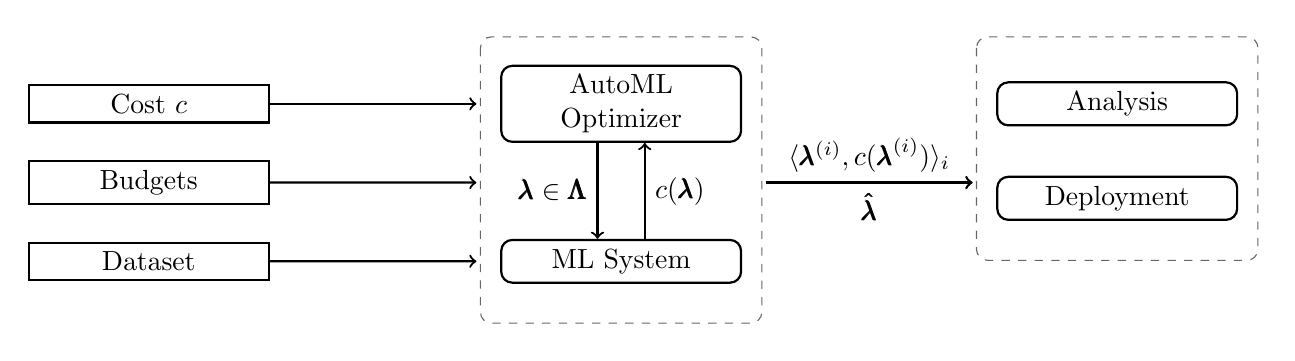
\begin{tikzpicture}[node distance=4cm, thick]
  \node (function) [data] {Cost $\cost$};
  \node (budgets) [data, below of=function, node distance=1cm] {Budgets};
  \node (dataset) [data, below of=budgets, node distance=1cm] {Dataset};
  
  \node (hb) [activity, right of=dataset, node distance=6cm, yshift=-0.0cm] {ML System};
  \node (kde) [activity, above of=hb, node distance=2cm] {AutoML Optimizer};
  
  \draw[myarrow] ($(kde.south)+(-0.3,0.0)$) -- ++(0.0,-0.6) node[left] {$\conf \in \pcs$} -- ($(hb.north)+(-0.3,+0.0)$);
  \draw[myarrow] ($(hb.north)+(0.3,+0.0)$) -- ++(0.0,0.6) node[right] {$\cost(\conf)$} -- ($(kde.south)+(0.3,0.0)$);
  
  \draw[myarrow] (function.east) -- ($(kde.west)+(-0.3,0.0)$);
  \draw[myarrow] (budgets.east) -- ($(kde.west)+(-0.3,-1.)$);
  \draw[myarrow] (dataset.east) -- ($(kde.west)+(-0.3,-2.)$);
  
  \node (perf) [activity, right of=kde, node distance=6.3cm] {Analysis};
  \node (budget) [activity, below of=perf, node distance=1.2cm] {Deployment};
  %\node (imp) [activity, below of=budget, node distance=1cm] {Space Analysis};
  
  \draw[myarrow] ($(kde.east)+(0.3,-1.)$) -- node[above] {$\langle \conf^{(i)}, \cost(\confI{i}) \rangle_i$} ($(perf.west)+(-0.3,-1.)$);
  \draw[myarrow] ($(kde.east)+(0.3,-1.)$) -- node[below] {$\finconf$} ($(perf.west)+(-0.3,-1.)$);
  
  \begin{pgfonlayer}{background}
  
  % Configuration Process
  \path (kde -| kde.west)+(-0.25,0.85) node (resUL) {};
  \path (hb.east |- hb.south)+(0.25,-0.5) node(resBR) {};
  \path [rounded corners, draw=black!60, dashed] (resUL) rectangle (resBR);
  \path (hb.east |- hb.south)+(-.5,-.3) node [text=black!60] {};
  
  \path (perf -| perf.west)+(-0.25,0.85) node (resUL) {};
  \path (budget.east |- budget.south)+(0.25,-0.5) node(resBR) {};
  \path [rounded corners, draw=black!60, dashed] (resUL) rectangle (resBR);
  \path (budget.east |- budget.south)+(-.5,-.3) node [text=black!60] {};
  
  \end{pgfonlayer}

\end{tikzpicture}
        }
      \end{center}
    \end{column}
  \end{columns}
\end{frame}

% \begin{frame}{Automate HPO}

%   \begin{columns}
%     \begin{column}{0.59\textwidth}

%       For AutoML the user only supplies \ldots
%       \begin{itemize}
%         \item dataset,
%         \item performance measure and
%         \item usually a time budget
%       \end{itemize}

%       To do HPO we need to \ldots
%       \begin{itemize}
%         \item preprocessing manually,
%         \item decide on an optimization algorithm,
%         \item an ML algorithm (to generate Inducer $\inducer$),
%         \item a search space $\pcs$ and
%         \item a resampling strategy to evaluate $\cost(\conf)$.
%       \end{itemize}

%       To build an AutoML System we have to make these choices automatically $\rightarrow$ Following slides.

%     \end{column}%
%     \begin{column}{0.4\textwidth}
%       \begin{center}
%         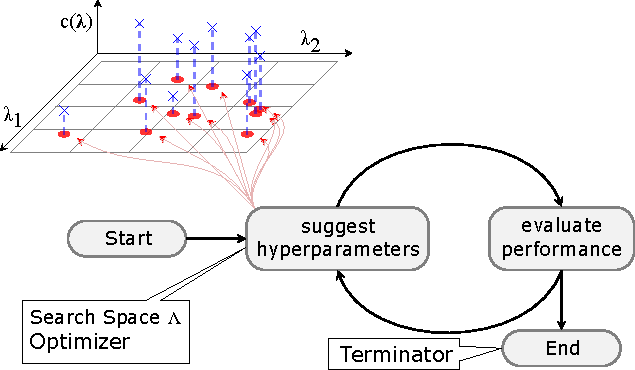
\includegraphics[width = \linewidth]{images/tuning.pdf}    
%       \end{center}
%     \end{column}
%   \end{columns}

% \end{frame}

\begin{frame}{Choice of Learning Algorithm}
  \begin{itemize}
    % \item A good AutoML System should consider more than one learning algorithm. More on that later.
    \item A plethora of learners exists, for different data sets different models
        are likely needed.
        
    \item Studies~\lit{{\href{https://jmlr.org/papers/volume15/delgado14a/delgado14a.pdf}{Fernandez-Delgado et al. 2014}}} and experience show:\\
        One these is often good -- on tabular data:
    \begin{itemize}
      \item penalized regression
      \item SVM
      \item gradient boosting
       \item random forests
     \item (neural networks)
  \end{itemize}
      % \item Random forests only beaten on few tabular datasets by current AutoML frameworks~\lit{\href{https://arxiv.org/abs/1907.00909}{Gijsbers et al., 2019}}.
      \item Example: Auto-Sklearn 2.0~ \lit{{\href{https://arxiv.org/pdf/2007.04074.pdf}{Feurer et al. 2020}}} uses: 
    \begin{itemize}
        \item extra trees 
         \item gradient boosting 
         \item passive aggressive 
        \item random forest 
        \item linear model
  \end{itemize}
    \end{itemize}
  % \end{itemize}
\end{frame}

\begin{frame}{Choice of Search Space for a Learning Algorithm}
  \begin{columns}
    \begin{column}{0.6\textwidth}
    % Which hyperparameters should we consider for a given learning algorithm?
    Ranges often selected based on experience
    \begin{itemize}
      \item See other AutoML frameworks: e.g.\ Auto-Sklearn 2.0~\lit{\href{https://arxiv.org/pdf/2007.04074.pdf}{Feurer et al. 2020}}
      \item Sensitivity analysis often does not exist for ML algorithms
      \item Check literature on specific ML algorithm
    \end{itemize}
    Options for automation:
    \begin{itemize}
      \item Use huge search space to cover all possibilities \\ 
            (combine with meta-learning for good initial design for Bayesian optimization)
      \item Use results of meta-experiments to obtain smaller search space that is estimated to work well.
      % \item FIXME: Wollte Bernd hier nochwas spezielles?
    \end{itemize}
    \end{column}%
    \begin{column}{0.4\textwidth}
      \begin{center}
        \only<1>{
          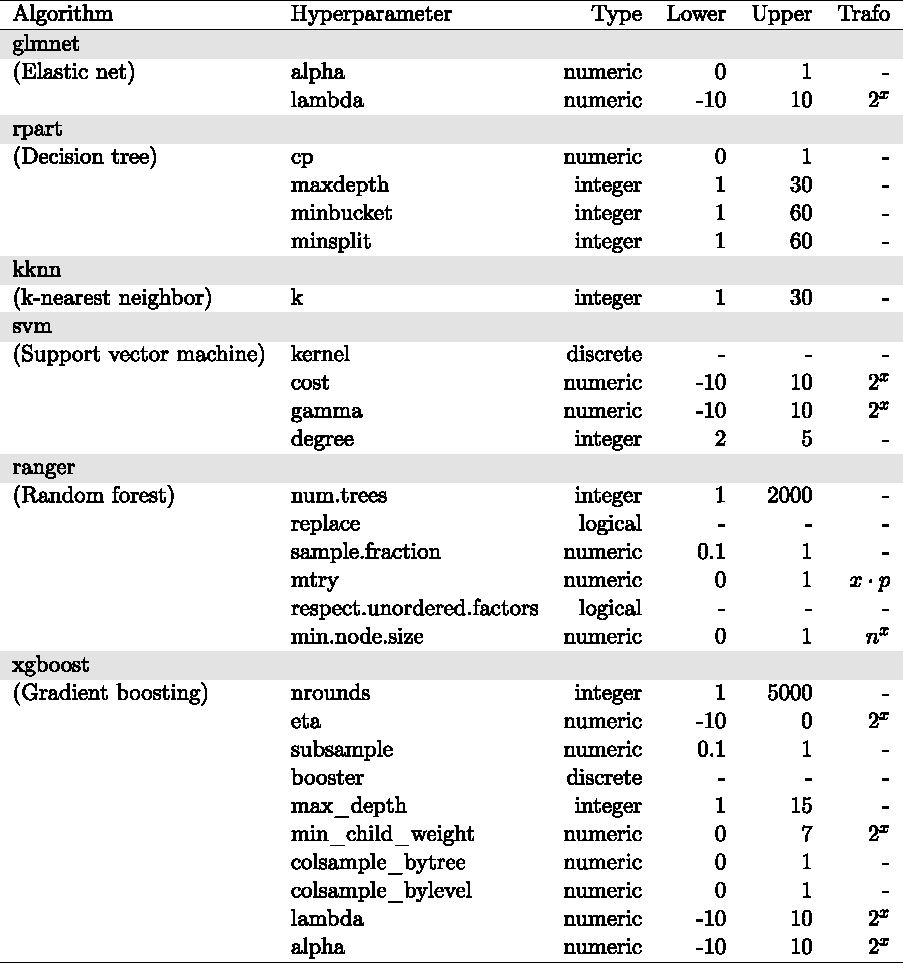
\includegraphics[width = 0.8\linewidth]{images/probst2019jmlr_tab1.pdf}
        }
        \only<2>{
          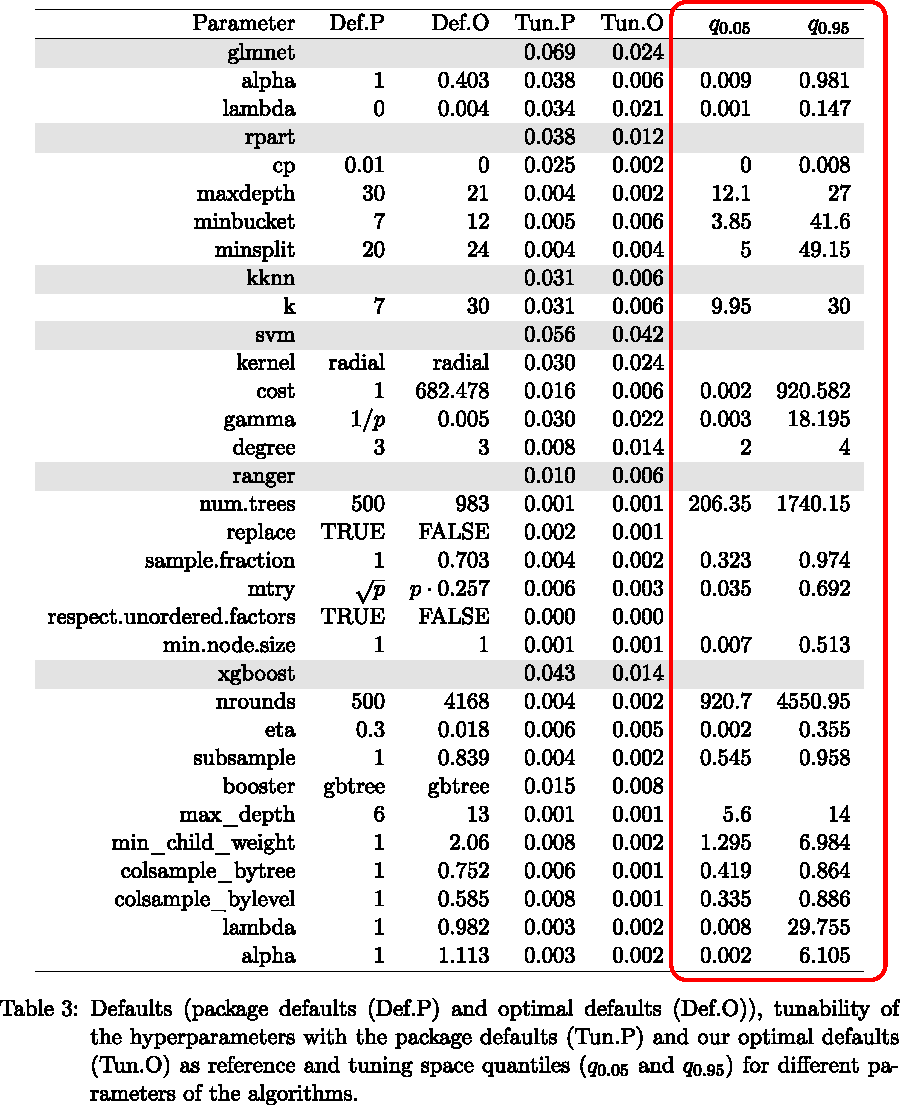
\includegraphics[width = 0.8\linewidth]{images/probst2019jmlr_tab3.pdf}   
        }


        {\tiny Taken from \lit{\href{https://www.jmlr.org/papers/volume20/18-444/18-444.pdf}{Probst et al. 2019 }}.}

      \end{center}
    \end{column}
  \end{columns}
\end{frame}

\begin{frame}{Choice of Resampling Strategy}
  
  For computation of generalization error / cost:
  \begin{equation*}
    \cost(\conf) = \frac{1}{k}\sum_{i = 1}^k \widehat{GE}_{\dataset_{\text{val}}^i}\left(\inducer(\dataset_{\text{train}}^i, \conf)\right)
  \end{equation*}
  % that defines the objective of the black-box optimization we need a resampling strategy.

  \vspace{1em}
  \begin{columns}
    \begin{column}{0.5\textwidth}
    Rules of thumb:
    \begin{itemize}
      \item Default: 10-fold CV ($k=10$)
      \item Huge datasets: holdout
      \item Tiny datasets: 10x10 repeated CV
      \item Stratification for imbalanced classes
    \end{itemize}
    \end{column}
    
    \begin{column}{0.5\textwidth}
 Watch out for this:       
    \begin{itemize}
      \item Small sample size situation because of imbalancies    
      \item Leave-one-object out
      \item Time dependencies
      \item A good AutoML system should let you customize resampling
          % errors here can mean: garbage in, garbvgae out
      \item Meta-learn good resampling strategy~\lit{\href{https://arxiv.org/abs/2007.04074}{Feurer et al., 2020}}
    \end{itemize}
    \end{column}
    \end{columns}
    
\end{frame}

\begin{frame}{Choice of Optimization Algorithm}
  Choose optimization algorithm based on \ldots
  \begin{itemize}
    \item complexity of search space / budget
    \item time-costs of evaluations
  \end{itemize}

  \vspace{0.5em}

  Complex search space
  \begin{itemize}
    \item[$\rightarrow$] EA with exploratory character, TPE, BO with RF 
    % \item[$\rightarrow$] Make use of Grey-Box Optimizers: Hyperband, BOHB
  \end{itemize}
  Numerical (lower-dim) search space and tight budget
  \begin{itemize}
    \item[$\rightarrow$] BO with GP
  \end{itemize}
  Expensive evals
  \begin{itemize}
    \item[$\rightarrow$] Hyperband, BOHB
  \end{itemize}
  Deep learning 
  \begin{itemize}
    \item[$\rightarrow$]Parametrize architectures, then HPO, see above
    \item[$\rightarrow$]NAS 
  \end{itemize}

\end{frame}



\begin{frame}{Preprocessing}
  \begin{columns}
    \begin{column}{0.5\textwidth} 
      Ideal AutoML systems should also optimize: 
      % the following steps wrt.\ given cost function:
      \begin{itemize}
        \item[\ding{55}] Data preprocessing
        \item[\ding{55}] Feature engineering
        \item[\ding{55}] Feature selection
          % \item Feature construction  
        \item[\ding{51}] Model training
      \end{itemize}
      \vspace{10em}
      {\tiny \ding{51} = already covered, \ding{55} = not covered so far}
    % We already know how to optimize the ml algorithm. How about the preprocessing steps?
    \end{column}%
    \begin{column}{0.5\textwidth}
      \begin{center}
        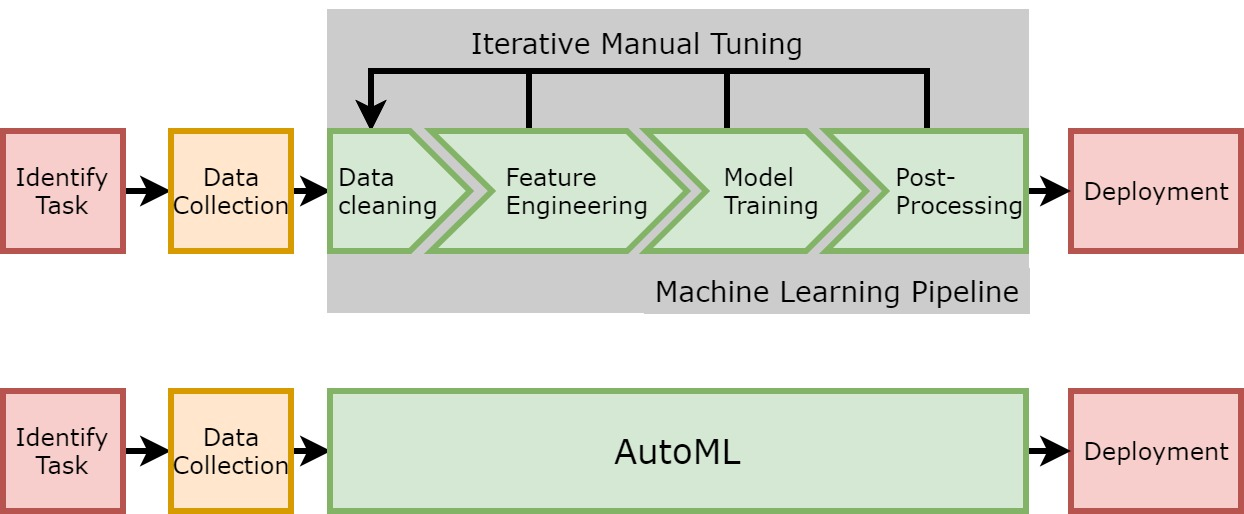
\includegraphics[width = \linewidth]{images/AutoMLPipeline.jpg}  
      \end{center}
    \end{column}
  \end{columns}
  
\end{frame}

\section{Common Preprocessing Steps}

\begin{frame}{Preprocessing capabilities differ heavily}
  \begin{columns}
    \begin{column}{0.6\textwidth}
      \vspace*{-1cm}
      \begin{center}
        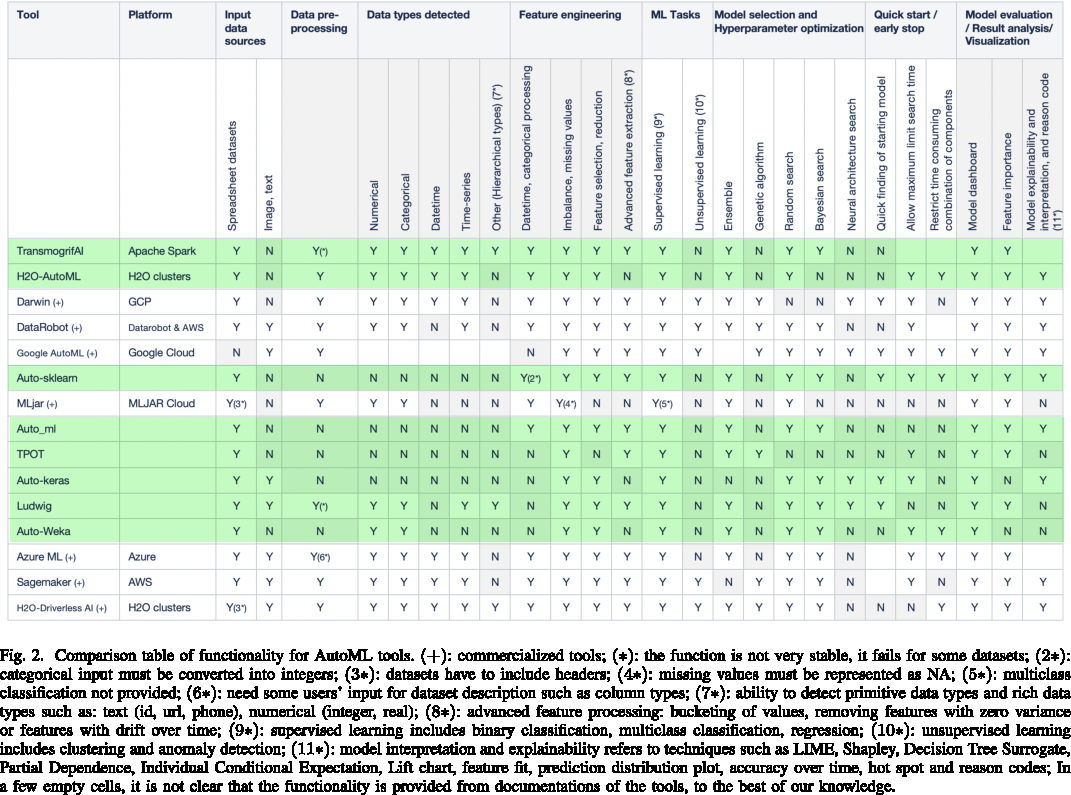
\includegraphics[width = \linewidth]{images/Truong2019Towards_fig2.pdf}
      \end{center}
    \end{column}%
    \begin{column}{0.4\textwidth}
    \small
      Taken from~\lit{\href{https://doi.org/10.1109/ICTAI.2019.00209}{Truong et al. 2019}}.
      \vspace{1em}

      Highlighted: Non-commercial AutoML frameworks

      \begin{itemize}
        \item Auto-detection of feature types: some
        \item Preprocess categoricals: some
        \item Imputation: all
        \item Class imbalance handling: all
      \end{itemize}
    \end{column}
  \end{columns}
\end{frame}

\begin{frame}{Cleaning}
  Data cleaning is hard to fully automate, but a few heuristics exist:
  \begin{itemize}
    \item Remove ID columns, columns with mostly unique values.
    \item Outlier detection 
    \item Detect time series or spatial data $\rightarrow$ 
        at the very least, evaluation and resampling needs to be adapted,
        but feature extraction likely as well
  \end{itemize}

  \vspace{1cm}

  It is highly unclear how much of this is required input by the user
  (last point is more or less task specification),
  and what should be automated by the system. 

\end{frame}

\begin{frame}{Categorical Features: Dummy Encoding}
  % Goals:
  \begin{itemize}
    \item Most simple encoding
    \item Works well with low cardinality categoricals
  \end{itemize}
  % ML algorithm does not support categorical features + few unique values $\rightarrow$ use dummy encoding.
  % Most simple technique to encode categ
  \begin{center}
    \resizebox{0.3\linewidth}{!}{
    \begin{tabular}{r|l|l}
    \hline
    SalePrice & Central.Air & Bldg.Type\\
    \hline
    189900 & Y & 1Fam\\
    \hline
    195500 & Y & 1Fam\\
    \hline
    213500 & Y & TwnhsE\\
    \hline
    191500 & Y & TwnhsE\\
    \hline
    236500 & Y & TwnhsE\\
    \hline
    \end{tabular}
    } \\
    
\begin{tikzpicture}
      %\useasboundingbox (-2,0);
      \node[single arrow,draw=black,fill=black!10,minimum height=1cm,shape border rotate=270] at (0,-1) {};
    \end{tikzpicture} \\
  \resizebox{0.9\linewidth}{!}{
    \begin{tabular}{r|r|r|r|r|r}
    \hline
    SalePrice & Y & Bldg.Type.2fmCon & Bldg.Type.Duplex & Bldg.Type.Twnhs & Bldg.Type.TwnhsE\\
    \hline
    189900 & 1 & 0 & 0 & 0 & 0\\
    \hline
    195500 & 1 & 0 & 0 & 0 & 0\\
    \hline
    213500 & 1 & 0 & 0 & 0 & 1\\
    \hline
    191500 & 1 & 0 & 0 & 0 & 1\\
    \hline
    236500 & 1 & 0 & 0 & 0 & 1\\
    \hline
    \end{tabular}
  }
  \end{center}
\end{frame}

\begin{frame}{Categorical Features: Target / Impact Encoding}
  \begin{itemize}
    \item Well known from CART
    \item Handles high cardinality categoricals, too
  \end{itemize}

  % Avoid high cardinality categorical features because they are problematic for all ML algorithms $\rightarrow$ use target encoding (also impact encoding).
  \begin{columns}
    \begin{column}{0.7\textwidth}


      \textbf{Goal}: Encodes each categorical $\bm{x}$ as a single numeric $\tilde{\bm{x}}$
      
      \vspace*{-0.5cm}  
      {\footnotesize
      \begin{align*}
      \text{Regression:} \operatorname{Impact}(x) &= \E(\bm{y} | x) - \E(\bm{y}) \\
      \text{Classification:} \operatorname{Impact}(x) &= \operatorname{logit}(P( y = \text{target} | x)) - \operatorname{logit}(P( y = \text{target}))
      \end{align*}
      }
      \vspace*{-0.5cm}  
      \begin{itemize}
      
        \item Needs regularization (through CV) to prevent target leakage \lit{\href{https://arxiv.org/pdf/1611.09477.pdf}{Zumel et al. 2019}}
        \item Advantage: Handles unknown categorical levels on test data
      \end{itemize}
      Alternatives: 
      \begin{itemize}
    \item factorization machines 
    \item clustering feature levels 
    \item feature hashing
      \end{itemize}
    \end{column}%
    \begin{column}{0.3\textwidth}
      \vspace{-1cm}
      \begin{center}
        %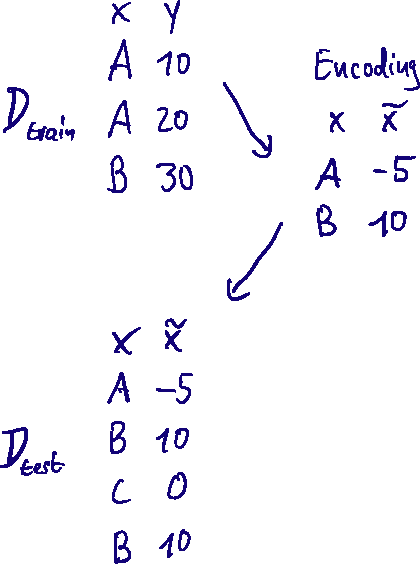
\includegraphics[width = \textwidth]{images/scetch_impact_encoding.pdf}
        \resizebox{0.8\columnwidth}{!}{
        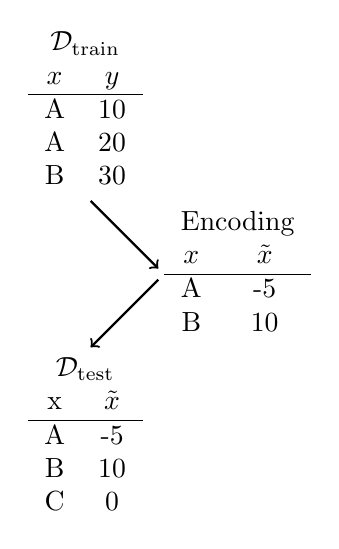
\begin{tikzpicture}
          \path
            (0,1) coordinate (A) node[above, inner sep=0] {
              \begin{tabular}{ c c }
                \multicolumn{2}{ c }{$\dataset_{\text{train}}$} \\
                %\hline
                $x$ & $y$  \\
                \hline
                A & 10 \\
                A & 20 \\
                B & 30 \\
              \end{tabular}
            }
            (0,-1) coordinate (B) node[below, inner sep=0] {
              \begin{tabular}{ c c }
                \multicolumn{2}{ c }{$\dataset_{\text{test}}$} \\
                %\hline
                x & $\tilde{x}$  \\
                \hline
                A & -5 \\
                B & 10 \\
                C & 0 \\
              \end{tabular}
            }
            (1,0) coordinate (C) node[right, inner sep=0] {
              \begin{tabular}{ c c }
                \multicolumn{2}{ c }{Encoding} \\
                %\hline
                $x$ & $\tilde{x}$  \\
                \hline
                A & -5 \\
                B & 10 \\
              \end{tabular}
            };
          %\draw[->] (A)--(B) (0,0) -- node[above]{}(C);
          \draw[myarrow, shorten <=0.1cm, shorten >=0.1cm] (A.south)--(C.north);
          \draw[myarrow, shorten <=0.1cm, shorten >=0.1cm] (C.south)--(B.north);
        \end{tikzpicture}
        }
      \end{center}
    \end{column}
  \end{columns}
\end{frame}

\begin{frame}{Common Preprocessing Steps: Missing Values}
  \begin{columns}
    \begin{column}{0.7\textwidth}
      \begin{itemize}
        \item Replace missings with imputed values, try not to 
            disturb distribution too much
        \item Examples: mean, median, mode, sample from histogram,
            predict value based on other features
        \item Additional factor column indicating missingness can help
            if NA-state carries information for target
        \item \emph{Out-Of-Range} works often well for tree-based techniques
            (RF and boosting!), saves extra missingness col
        \item For inference, simple imputation is often shunned, 
            and multiple, model-based imputation recommended; 
            for prediction naive imputation often works remarkably well

      \end{itemize}
    \end{column}%
    \begin{column}{0.3\textwidth}
            \vspace{-0.65cm}
      \begin{center}
        %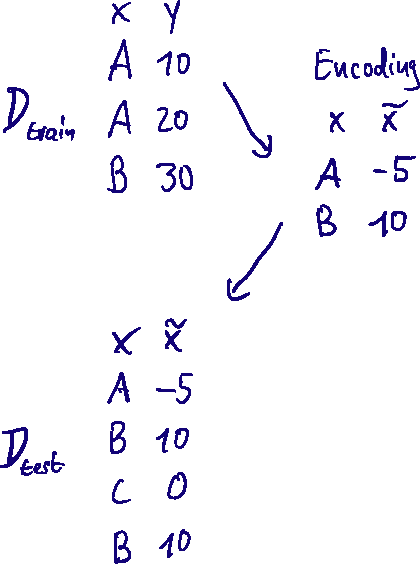
\includegraphics[width = \textwidth]{images/scetch_impact_encoding.pdf}
        \resizebox{0.9\columnwidth}{!}{
        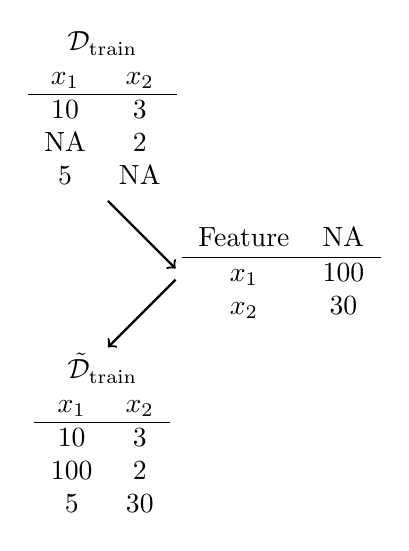
\begin{tikzpicture}
          \path
            (0,1) coordinate (A) node[above, inner sep=0] {
              \begin{tabular}{ c c }
                \multicolumn{2}{ c }{$\dataset_{\text{train}}$} \\
                %\hline
                $x_1$ & $x_2$  \\
                \hline
                10 & 3 \\
                NA & 2 \\
                5  & NA \\
              \end{tabular}
            }
            (0,-1) coordinate (B) node[below, inner sep=0] {
              \begin{tabular}{ c c }
                \multicolumn{2}{ c }{$\tilde{\dataset}_{\text{train}}$} \\
                %\hline
                $x_1$ & $x_2$  \\
                \hline
                10  & 3 \\
                100 & 2 \\
                5   & 30 \\
              \end{tabular}
            }
            (1,0) coordinate (C) node[right, inner sep=0] {
              \begin{tabular}{ c c }
                %\multicolumn{2}{ c }{Replacements} \\
                %\hline
                Feature & NA  \\
                \hline
                $x_1$ & 100 \\
                $x_2$ & 30 \\
              \end{tabular}
            };
          %\draw[->] (A)--(B) (0,0) -- node[above]{}(C);
          \draw[myarrow, shorten <=0.1cm, shorten >=0.1cm] (A.south)--(C.north);
          \draw[myarrow, shorten <=0.1cm, shorten >=0.1cm] (C.south)--(B.north);
        \end{tikzpicture}
        }
        \end{center}
        {\footnotesize
        \emph{Out of range} imputation
        }
    \end{column}
  \end{columns}
\end{frame}

\begin{frame}{Feature Selection}
    \begin{columns}
      \begin{column}{0.4\textwidth}
        \begin{itemize}
        
          \item Filter; for ultra-highdim tasks
          \item Stepwise / wrapper methods; 
              % m: Needs to be applied on the whole pipeline (impractical!)
          seldom increases performance when well-regularized 
              learners are used, but quite expensive 
          \item Embedded: CART, lasso, \ldots 
          \item Selection interesting when predictive performance vs. sparseness
              should be optimized $\rightarrow$ multi-criteria optimization
            \item Combined feature selection and HPO: \lit{\href{https://arxiv.org/pdf/1912.12912.pdf}{Binder et al. 2020}}
            
        \end{itemize}
      \end{column}%
      \begin{column}{0.6\textwidth}
        \begin{center}
          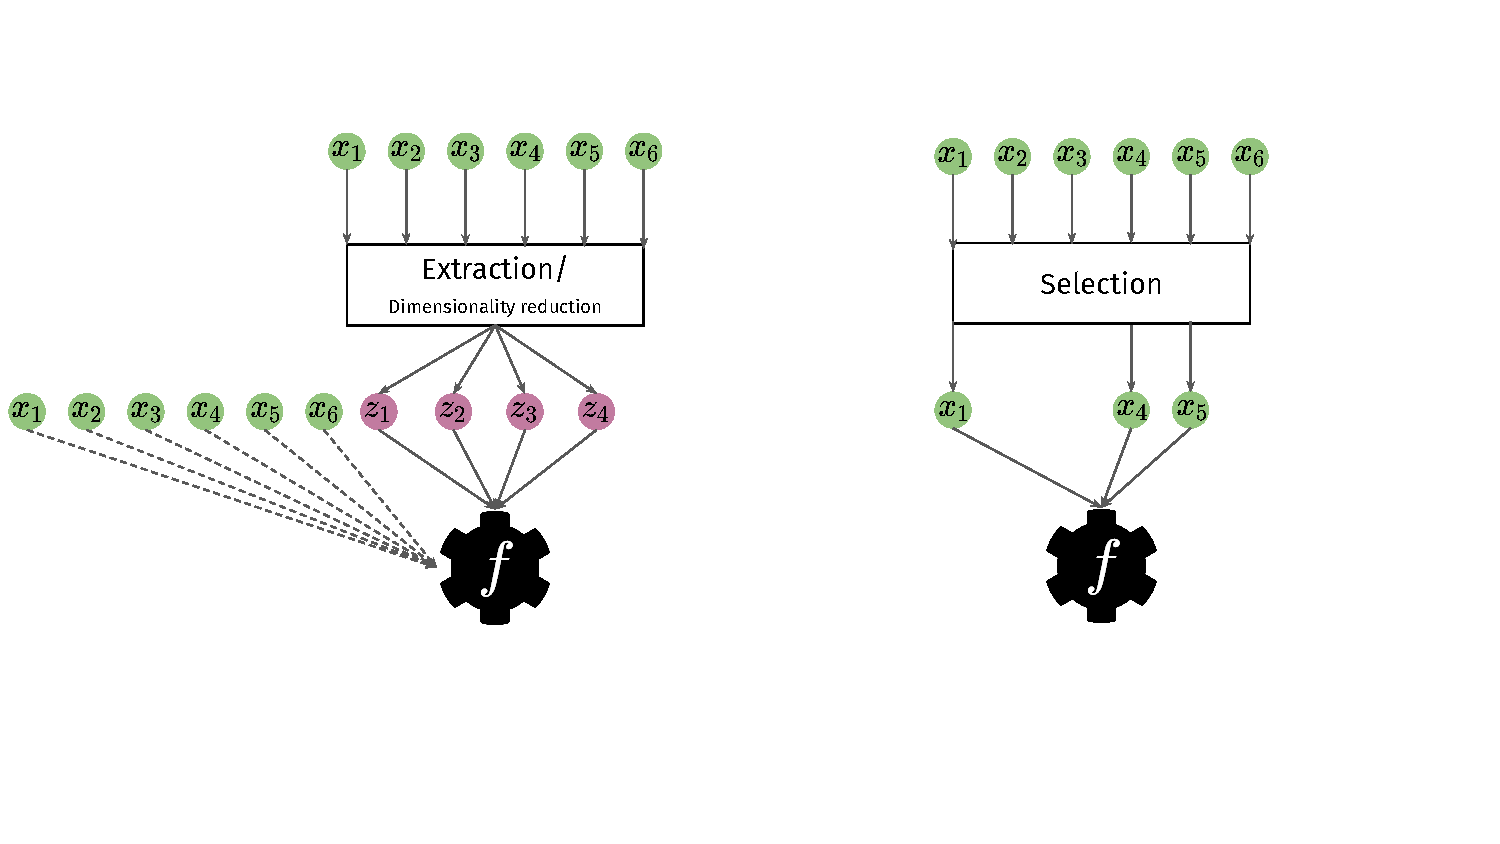
\includegraphics[width=0.35\textwidth, trim=450 100 110 60, clip]{images/feat_extr_vs_selection.pdf}%
          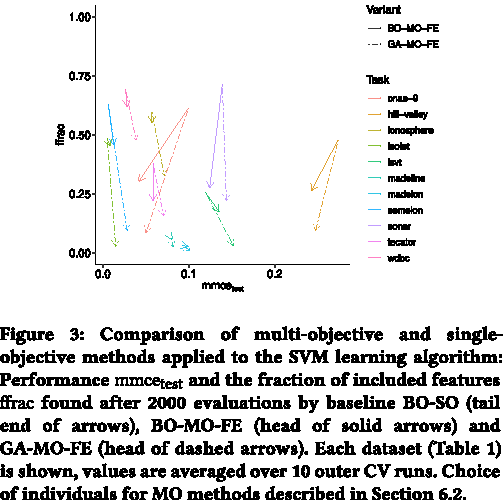
\includegraphics[width=0.55\linewidth]{images/Binder2020multiobjective_fig3.pdf}


          {\tiny \hfill Taken from \lit{\href{https://arxiv.org/pdf/1912.12912.pdf}{Binder et al. 2020}}.}

        \end{center}
      \end{column}
    \end{columns}
    
\end{frame}

\begin{frame}{Common Feature Construction Methods}
  \begin{columns}
    \begin{column}{0.6\textwidth}
    Reduction:
    \begin{itemize}
      \item PCA, ICA, autoencoder
    \end{itemize}

    Feature extraction:
    \begin{itemize}
      \item Polynomial features: $x_j \longrightarrow x_j, x_j^2, x_j^3, ...$
      \item Interactions: $x_j, x_k \longrightarrow x_j, x_k, x_j \cdot x_k$
    \end{itemize}

    Feature generation:
    \begin{itemize}
      \item Transform to ``circular'' features (month, day) \\
      e.g.\ $\tilde x_1 = sin(2\pi \cdot x /24)$ and $\tilde x_2 = cos(2\pi \cdot x /24)$
    \end{itemize}
    
    Combine with external data:
    \begin{itemize}
      \item names $\longrightarrow$ gender, ethnicity, age
      \item home address $\longrightarrow$ household income
      \item location + date $\longrightarrow$ weather
    \end{itemize}

    \end{column}%
    \begin{column}{0.4\textwidth}
      \begin{center}
        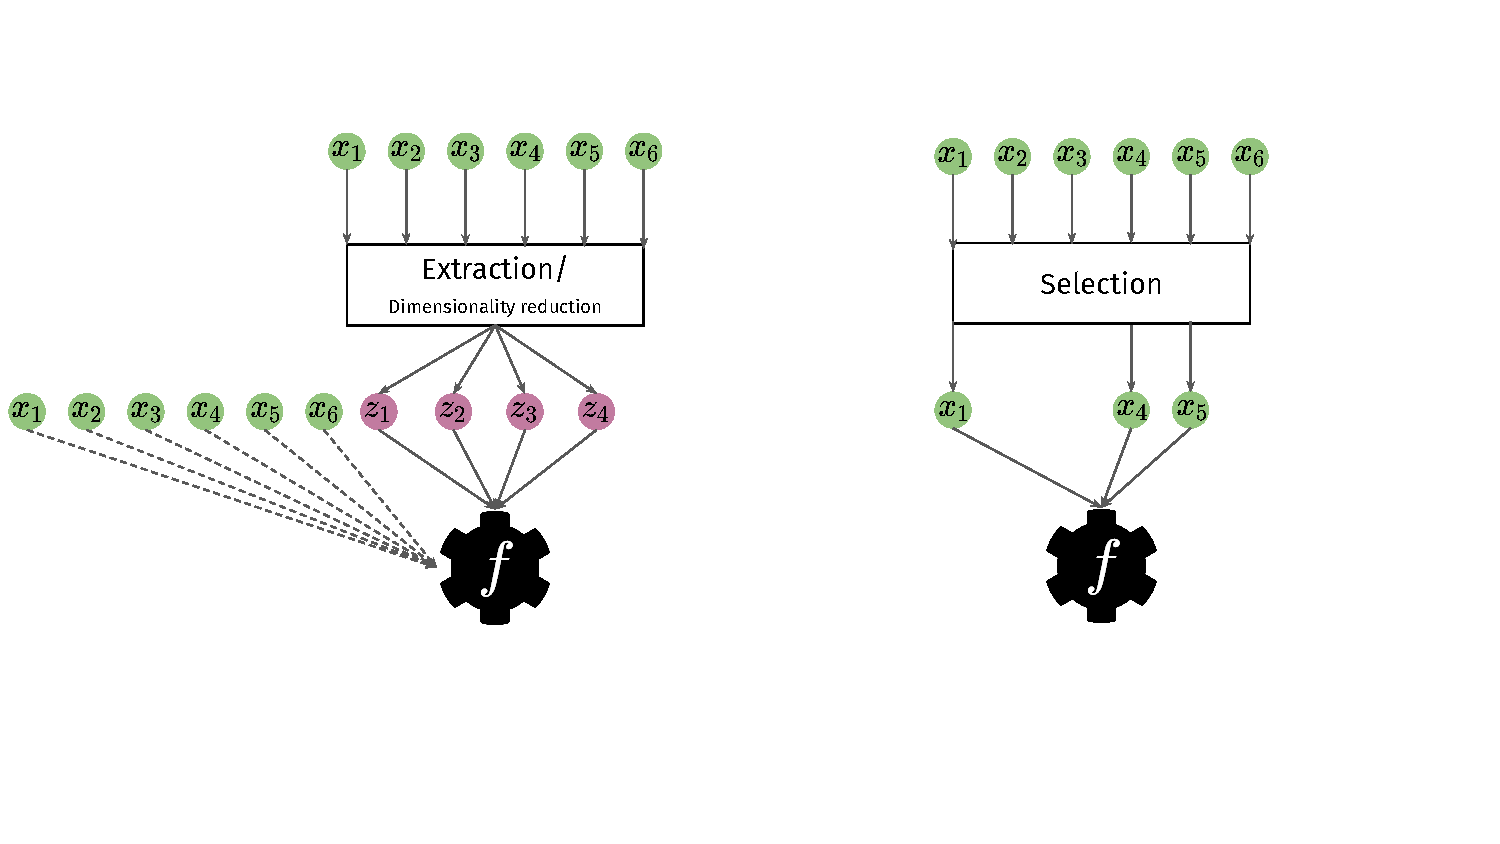
\includegraphics[width= \textwidth, trim=0 100 390 60, clip]{images/feat_extr_vs_selection.pdf}
      \end{center}
    \end{column}
  \end{columns}
    
\end{frame}


\begin{frame}{Imbalanced Classes}
  \begin{itemize}
    \item Oversampling of minority class
    \item Seldom: undersampling of majority class
    \item Intelligent oversampling strategies which create
        synthetic observations (SMOTE) 
        % can lead to improvement in predictive accuracy
  \end{itemize}
  %FIXME: HIER SOLLTE SMOTE PIC REIN
      \begin{center}
        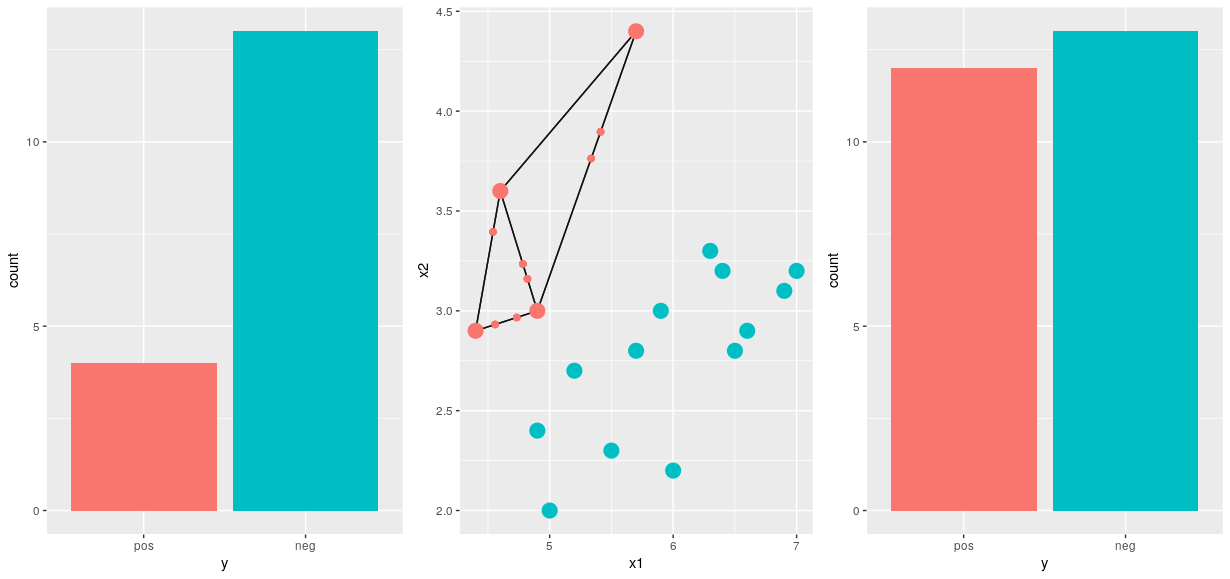
\includegraphics[width= 0.7\textwidth]{images/smote.png}
      \end{center}
\end{frame}

\section{Practical Problems}

\begin{frame}{Practical Problems: Stability}
  AutoML system should: 
  \begin{itemize}
    \item never fail to return a result
    \item terminate within a given time
    \item save intermediate results and allow to continue
  \end{itemize}

  Failure points:
  \begin{itemize}
    \item optimizer can crash (e.g.\ GP in BO) 
        % $\longrightarrow$ return intermediate result, continue with warmstart / random search
    \item training can crash (e.g. segfault) 
    \item training can run "forever" 
    % \item prediction can crash $\longrightarrow$ use prediction of fallback learner
  \end{itemize}

  Ways out
  \begin{itemize}
    \item Encapsulate train/predict in separate process from HPO
    \item Ressource limit time and memory of that process by OS
    \item If learner crashes, run robust fallback (constant predictor)   
    \item Use "robust" HPO, run random config as last resort if proposal fails (exploration)
  \end{itemize}

\end{frame}

\begin{frame}{Practical Problems: Parallelization}
  Parallelization should allow:
  \begin{itemize}
    \item multiple cores
    \item multiple nodes 
  \end{itemize}

  Possible parallelization levels:
  \begin{itemize}
    \item training of learner (threading / GPU)
    \item resampling
    \item eval configurations (batch proposal of HPO)
  \end{itemize}

  Possible problems:
  \begin{itemize}
    \item Sequential nature of HPO algorithms (e.g.\ BO)
    \item Heterogeneous runtimes cause idling $\longrightarrow$ 
        asynchronous HPO attractive, but more complex
    \item Main memory or CPU-cache becomes bottleneck
    \item Communication between workers
  \end{itemize}

\end{frame}


\section{Combined Preprocessing and Model Building: Pipelining}

\begin{frame}{Linear Pipelining}

  % Most preprocessing steps have parameters or can be switched on/off in the pipeline.

  % \vspace{1em}

  % \textbf{Goal:} Find optimal preprocessing parameters $\rightarrow$ HPO

  \begin{columns}
    \begin{column}{0.5\textwidth}
    \begin{itemize}
      \item Applying preprocessing to the whole dataset leads to data leakage
      \item Preprocessing should have train and predict steps, too
      \item Can add it to learner, and embed it in CV    
      \item Surprise: Preproc has hyperparameters 
      \item Optimize pipeline jointly: $\pcs = \pcs_{\text{preproc}} \times \pcs_\inducer$ 
      \item Still HPO, not much different than for single learner
      \item $\pcs$ "simply" of higher dimension
    \end{itemize}
    \end{column}%
    \begin{column}{0.5\textwidth}
      \begin{center}
        \includegraphics[page=19, width=\textwidth, trim=20 60 30 35, clip]{images/mlr3Pipelines_graphics}
      \end{center}
    \end{column}
  \end{columns}

\end{frame}

\begin{frame}{Nonlinear Pipelines}

  \begin{columns}
    \begin{column}{0.6\textwidth}
      Ideal to let HPO choose automatically:
      \begin{itemize}
      \item preprocessing
      \item feature extraction   
      \item learner
      \item[$\rightarrow$] $\pcs$ becomes hierarchical search space!
      \end{itemize}
      
      \vspace*{0.5em}

      Suitable optimizers:
      \begin{itemize}
        \item TPE
        \item Random search, hyperband with sampler that follows the hierarchy
        \item BO with RF (imputation or hierarchical trees)
        \item Evolutionary approaches (similar to NAS)
      \end{itemize}

    \end{column}%
    \begin{column}{0.4\textwidth}
      \begin{center}
        %\includegraphics[page=7, width=\textwidth, trim=160 0 30 160, clip]{images/mlr3Pipelines_graphics}
        %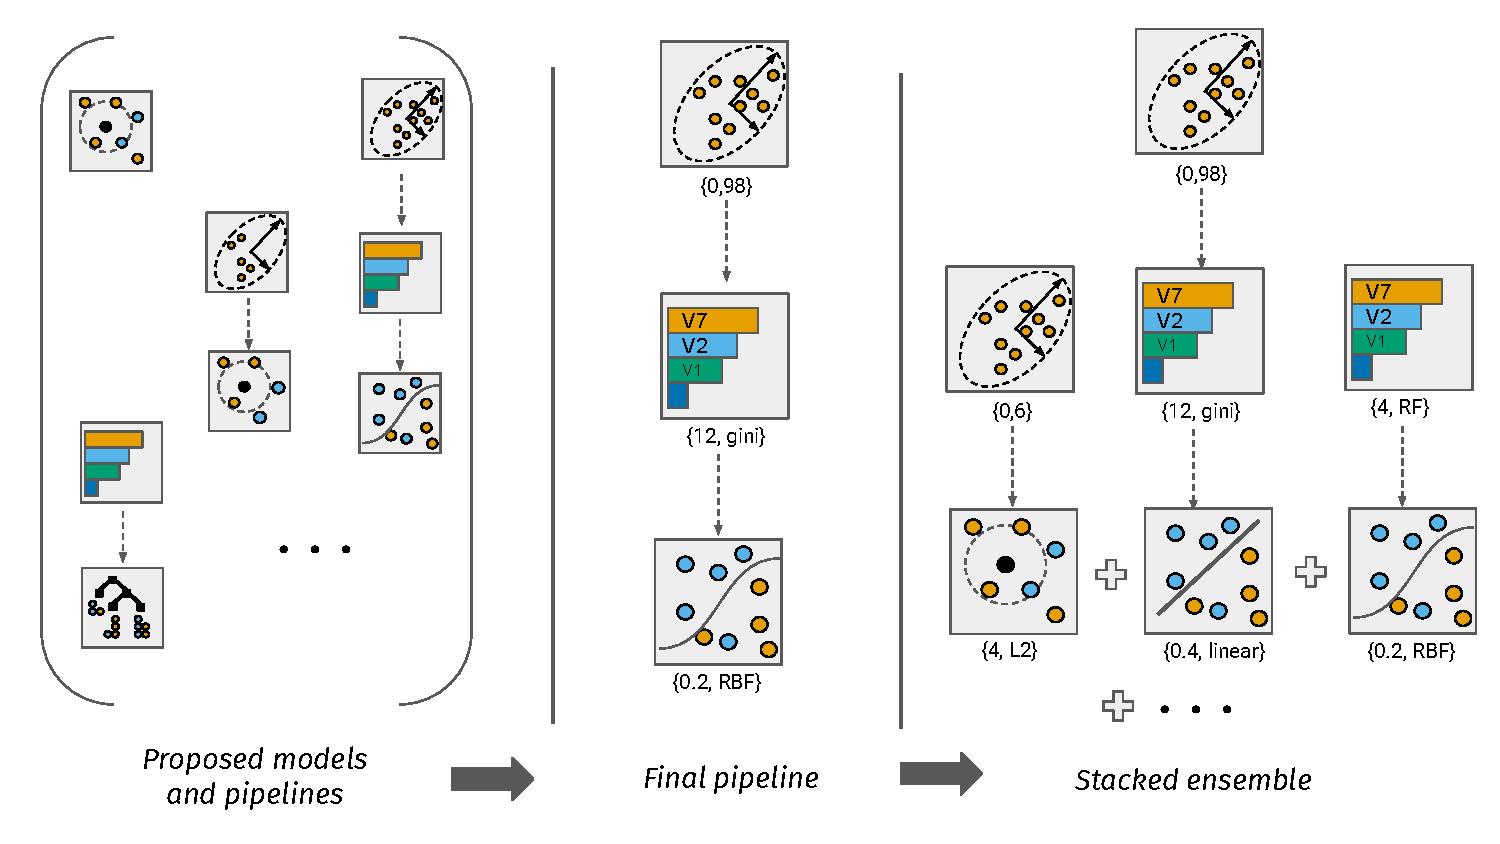
\includegraphics[width = \textwidth]{images/stacking.pdf}
        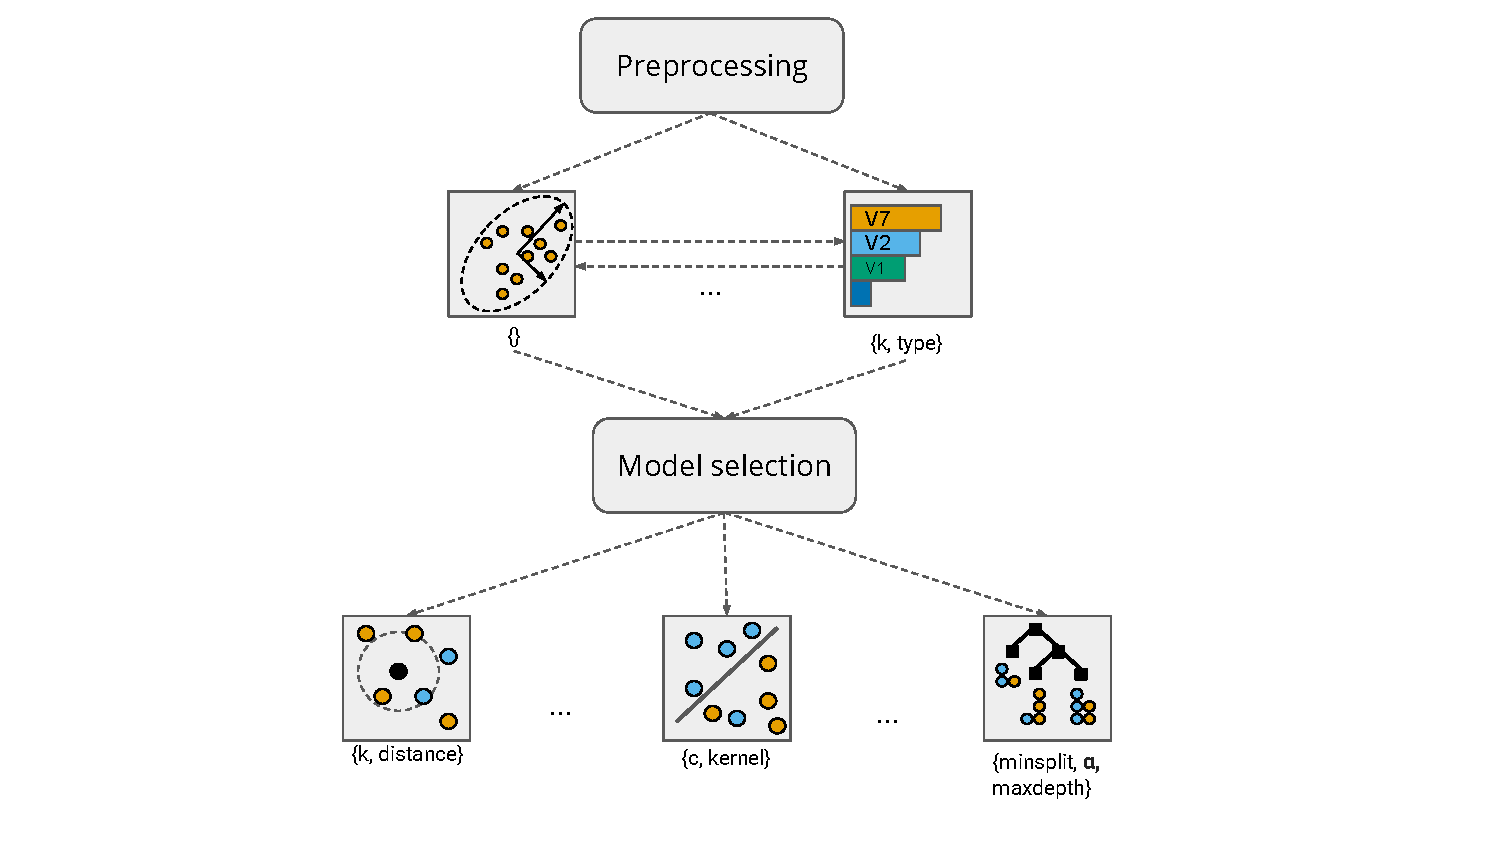
\includegraphics[width = \textwidth, trim=160 0 160 5, clip]{images/dag.pdf}
      \end{center}
    \end{column}
  \end{columns}
\end{frame}

\begin{frame}{Obtaining Final Model}


  Options:
  \begin{itemize}
    \item Choose the optimal path as linear pipeline.
    \item Build ensemble of best configurations\\ 
        (e.g. \lit{\href{https://papers.nips.cc/paper/2015/hash/11d0e6287202fced83f79975ec59a3a6-Abstract.html}{Feurer et al., NIPS 2015}}, \lit{\href{https://www.automl.org/wp-content/uploads/2020/07/AutoML_2020_paper_61.pdf}{LeDell and Poirier. 2020}}).
  \end{itemize}
  \begin{center}
    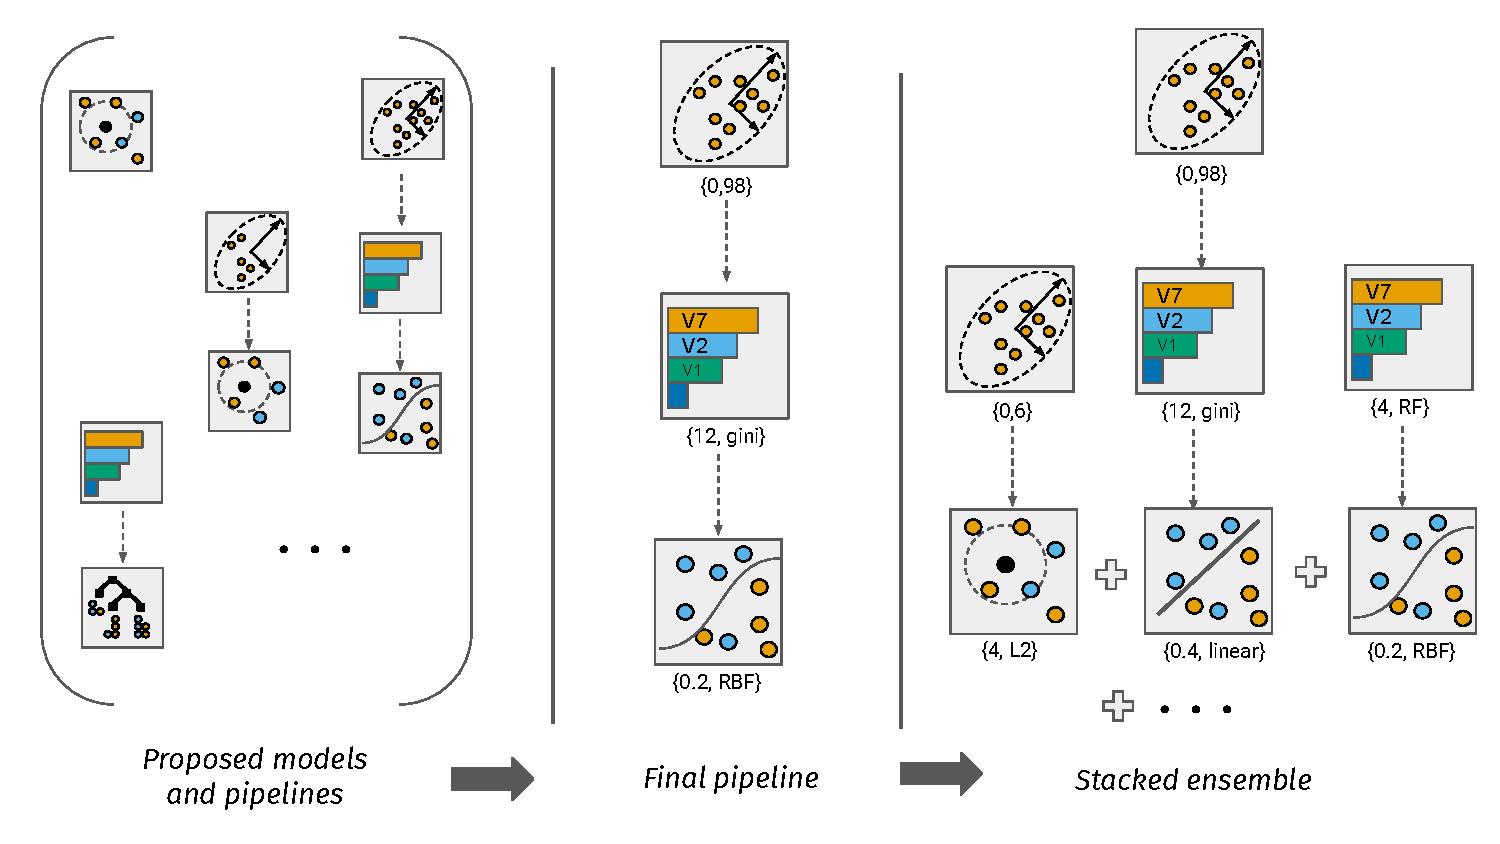
\includegraphics[width = 0.60\textwidth]{images/stacking.pdf}
  \end{center}
    
\end{frame}

\begin{frame}{Current Benchmark on Tabular Data}
  \begin{columns}
    \begin{column}{0.43\textwidth}
      \vspace{-0.7cm}

   
      \begin{center}
        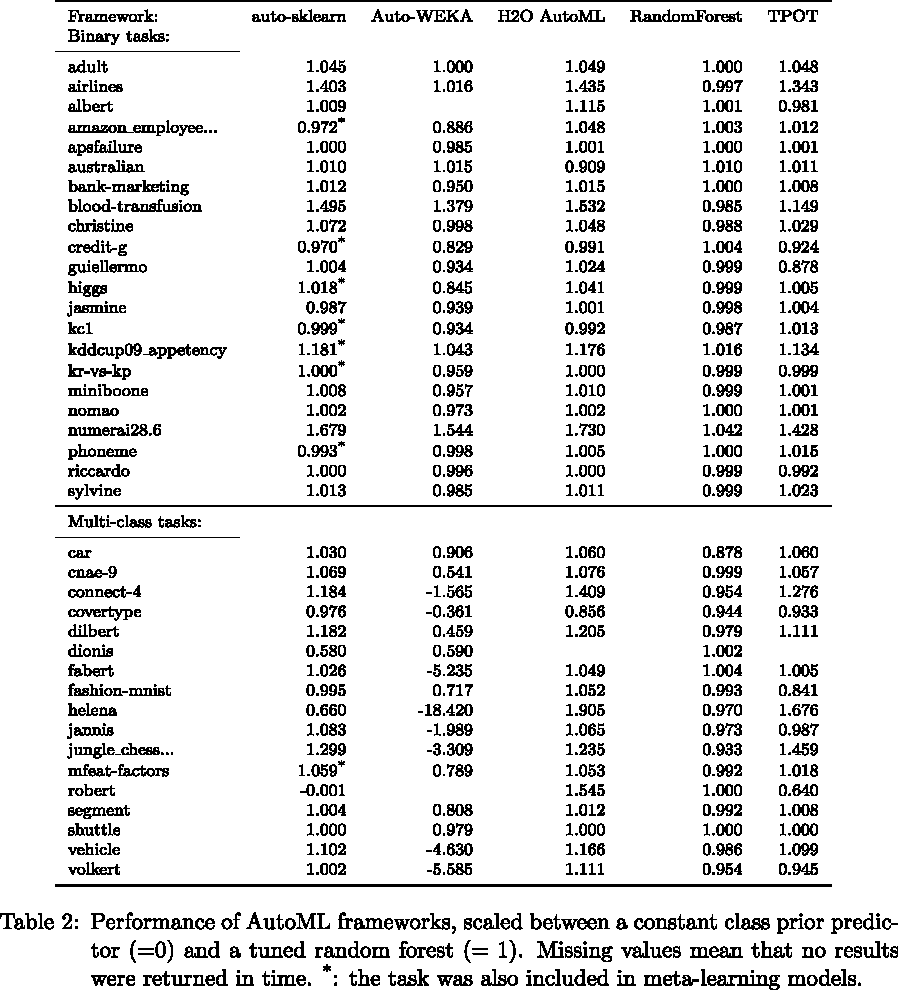
\includegraphics[width = \textwidth]{images/gijsbers_open_2019_tab2.pdf}
      \end{center}
    \end{column}%
    \begin{column}{0.57\textwidth}
      Table taken from \lit{\href{http://arxiv.org/abs/1907.00909}{Gijsbers et al., 2019}}.

      \begin{itemize}
        \item On some datasets AutoML yields big performance improvements
        \item On many datasets RF is equally good
        \item Need more and diverse benchmarks
      \end{itemize}

    \end{column}
  \end{columns}
\end{frame}

% \begin{frame}[containsverbatim,allowframebreaks]{Software}

% \begin{itemize}
%   \item DataRobot (comercial, gui)
%   \item H20.ai (comercial but open source, r, python)
%   \item TPOT, Tree-based Pipeline Optimization Tool  (2016-cont, open source, evolutionary approach) % show plot https://github.com/EpistasisLab/tpot
%   \item AutoWEKA (2016, open source)
%   \item mlr3automl (2020, prelim)
%   \item Hyperopt-Sklearn (2014-cont) Only HPO
%   \item Auto-Sklearn (2.0) (2015-cont) BO, ensembles, meta-learning
% \end{itemize}

% \end{frame}



\end{document}
